\documentclass[UTF8,ctexart,a4paper,11pt,openany]{article}
\usepackage[slantfont,boldfont]{xeCJK}
\usepackage{fontspec}
\usepackage{ctex}

\setCJKmainfont{SimSun}%[BoldFont=SimHei] %去掉注释:bf字体为黑体

\setsansfont{SimHei}
\setCJKsansfont{SimHei}

\xeCJKsetcharclass{"2160}{"2470}{1}% 1: CJK
\xeCJKsetup{AutoFallBack=true}
\setCJKfallbackfamilyfont{\CJKrmdefault}{SimSun.ttf}

%\setmainfont{Times New Roman}     %去掉注释:Times new roman字体
%\usepackage{mathptmx}             %去掉注释:Times new roman字体

\usepackage{mathtools}
\usepackage{amsmath}
\usepackage{amsfonts}
\usepackage{amssymb}
\usepackage{amsthm}
\usepackage[T1]{fontenc}
\usepackage{indentfirst} %段首空两格

\usepackage{graphicx}
\usepackage{geometry}
\usepackage{latexsym}
\usepackage{fancyhdr}
\usepackage{epstopdf}
%\usepackage{pifont}
%\usepackage[perpage,symbol*]{footmisc}
\usepackage{titlesec}
\usepackage{setspace}
\usepackage{enumerate}
\usepackage{enumitem}
\usepackage{multicol}
\usepackage{url}
\usepackage{exscale}
\usepackage{ulem}
\usepackage{relsize}
\usepackage{mathrsfs}
\usepackage{tikz}
\usepackage{wrapfig}
\usepackage{framed}
\usepackage{bm}
%\usepackage{pstricks,pst-node,multido,ifthen,calc}
\usepackage[all]{xy}
\usepackage{extarrows}
%\usepackage[backref]{hyperref}
\usepackage{hyperref}
\usepackage{stfloats} %插图的时候不分页

\setlength{\parindent}{2em} %段首空两格
\linespread{1.2}
\usepackage{listings}
\usepackage{xcolor}
\usepackage{algorithm}
\usepackage{algorithmicx}
\usepackage{algpseudocode}
\usepackage{mdframed}
\usepackage{extarrows}
\usepackage{diagbox}
\usepackage{makecell}

\theoremstyle{definition}
\mdfdefinestyle{theoremstyle}{%
linecolor=green!40,linewidth=.5pt,%
backgroundcolor=green!10,
skipabove=8pt,
skipbelow=5pt,
innerleftmargin=7pt,
innerrightmargin=7pt,
frametitlerule=true,%
frametitlerulewidth=.5pt,
frametitlebackgroundcolor=green!35,
frametitleaboveskip=0pt,
frametitlebelowskip=0pt,
innertopmargin=.4\baselineskip,
innerbottommargin=.4\baselineskip,
shadow=true,shadowsize=3pt,shadowcolor=black!20,
%theoremseparator={\hspace{1pt}},
theoremseparator={.},
nobreak=true,
}


\everymath{\displaystyle}

\newtheorem{definition}{\hspace{2em}定义}[section]
\newtheorem{axiom}{\hspace{2em}公理}

\mdtheorem[style=theoremstyle]{theorem}{定理}
\mdtheorem[style=theoremstyle]{example}{例}
\mdtheorem[style=theoremstyle]{exercise}{问题}
\newtheorem{lemma}[theorem]{\hspace{2em}引理}
\newtheorem{corollary}[theorem]{\hspace{2em}推论}

\newcommand*{\QED}{\hfill\ensuremath{\square}}
\newcommand*{\rmk}{\textbf{注:}}
\renewcommand*{\proof}{\textbf{证明:}}
\newcommand*{\tips}{\textbf{提示:}}
\newcommand*{\hard}{\textbf{\color{red}(难)}}
\newcommand*{\eqsmall}{\setlength\abovedisplayskip{1pt}\setlength\belowdisplayskip{1pt}}
\geometry{left=2cm,right=2cm,top=2cm,bottom=2cm}
% \title{数值分析上机报告(示例}
% \author{Fiddie}
\pagestyle{fancy}
\fancyfoot[C]{}
\fancyhead[RO]{ \thepage}
\fancyhead[LE]{\thepage  }
% \fancyhead[RE]{\rightmark (By Fiddie)}
% \fancyhead[LO]{\leftmark (By Fiddie)}
\titleformat{\chapter}{\centering\huge\bfseries}{第\,\thechapter\,章}{1em}{} %更改标题样式
\titleformat{\section}{\bfseries\Large}{$\S$\,\thesection\,}{1em}{} %更改标题样式
\titlespacing*{\chapter}{0pt}{9pt}{0pt} %调整标题间距
\setenumerate[1]{itemsep=0pt,partopsep=0pt,parsep=\parskip,topsep=0pt} %设置enumerate行间距
\setenumerate[2]{itemsep=0pt,partopsep=0pt,parsep=\parskip,topsep=0pt} %设置enumerate行间距
\setitemize[1]{itemsep=0pt,partopsep=0pt,parsep=\parskip,topsep=0pt} % 设置itemize行间距
\setlist[enumerate,2]{label=(\arabic*),topsep=0mm,itemsep=0mm,partopsep=0mm,parsep=\parskip}
    % 设置二层枚举为(1)样式
    
\newfontfamily\hei{SimHei}
\newcommand\textcf[1]{\textbf{\textsf{\hei{#1}}}}

\newcommand\e{\leftarrow}
%\renewcommand{\bibname}{参考文献}

\begin{document}
\begin{center}
{\huge \textbf{数值分析第3次上机作业}}

{\large 学号:221840189,姓名:王晨光}
\end{center}
\section{问题}
    考虑函数$$R(x)=\frac{1}{1+x^2},$$利用下列条件做插值逼近,并与$R(x)$的图像比较.
\section{问题一}
    \subsection{问题}
    用节点$$x_i=5cos(\frac{2i+1}{42}\pi),i=0,1,...,20.$$画出20次Lagrange插值多项式的图像;
    \subsection{算法思路}
    利用Lagrange插值公式:
\[
    p_n(x)=\sum_{i=0}^n f(x_i)l_i(x)
\]
其中
$$
    l_i(x)=\prod_{\substack {j=0, \\ j\neq i}}^n \dfrac{x-x_j}{x_i-x_j},\quad i=0,1,\cdots,n
$$
这是Lagrange基本多项式.\\ \indent
    由此在编程时只需记录下插值基点以及对应的函数值,就可以通过Python的Scipy库中的\texttt{inter\\polate.lagrange}函数构造出Lagrange插值多项式.
    \begin{algorithm}[H]
        \caption{Lagrange插值多项式}
        \begin{algorithmic}[1]
            \For {$i$ from 0 to 20}
                \State $x_i\e 5cos(\frac{2i+1}{42}\pi)$
                \State $y_i\e \frac{1}{1+x_i^2}$
            \EndFor
            \State $x=-5$ 
            \For {$i$ from 1 to 2000}
                \For {$j$ from 0 to 20}
                    \For {$k$ from 0 to 20}
                        \If {$j\neq k$}
                            \State $T(j,i)\e \dfrac{x-x_k}{x_j-x_k}T(j,i)$
                        \EndIf
                    \EndFor
                \EndFor
                \State $x\e x+0.005$
            \EndFor
            \State $x=-5$
            \For {$i$ from 1 to 2000}
                \For {$j$ from 0 to 20}
                    \State $f(x)\e y_j T(j,i)+f(x)$
                \EndFor
                \State $x\e x+0.005$
            \EndFor
            \State \Return $f$ 
        \end{algorithmic}
    \end{algorithm}
    具体的代码由Python实现. 由于Python作图是通过大量的散点做出的,故在实际的作图中选取了横坐标间距为0.005个单位的点来作图(共2000个),这样在兼顾时间复杂度的同时,保证了图像具有一定的平滑度.\\ \indent
    同样由于Python作图是通过大量的散点做出的,故我们不需要给出多项式的具体表达式,只需要计算Lagrange多项式在2000个作图点的取值即可(后四个作图的思路同样如此,故再不赘述,并省略处理2000个采样点的伪代码过程).
    \subsection{结果分析}%重点(误差图、结果图、分析算法的收敛性(速度)、内存使用(时间、空间)、计算量、稳定性
    \begin{figure}[H]
        \centering
        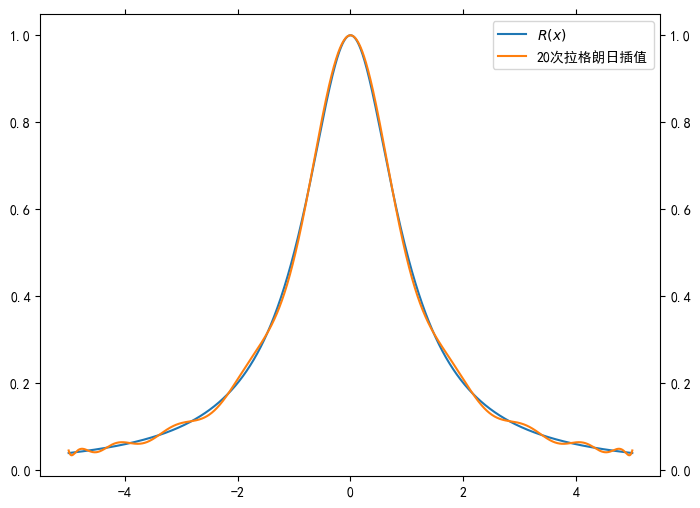
\includegraphics{pics/P3.1.png}
        \caption{问题一图像对比}
        \label{graph:1}
        \end{figure}
    可以看出,在图像中间部分Lagrange插值多项式逼近较好,而在靠近两端的部分出现了一些震荡. 值得一提的是,虽然使用插值多项式次数较高(20次),但由于选择插值基点间距不是均匀的,所以并未出现课本所说的Runge现象.
\section{问题二} 
    \subsection{问题}
    用等距节点$x_i=-5+i, i=0,1,...,10.$画出10次Newton插值多项式的图像;
    \subsection{算法思路}
    对于Newton插值多项式,首先需要构造出n阶均差表,即一个$n\times n$的矩阵,其对角线上的元素即为所需的系数.

    由于Newton插值多项式与Lagrange插值多项式的最终表达式相同,同样可以通过Python的Scipy库中的\texttt{interpolate.lagrange}函数构造出Newton插值多项式.
    \begin{algorithm}[H]
        \caption{Newton插值多项式}
        \begin{algorithmic}[1]
            \For {$i$ from 1 to 11}
                \State $x_i\e -5+ i -1$
                \State $Q_{i+1,1}\e \frac{1}{1+x_i^2}$
            \EndFor
            \For {$j$ from 2 to 11}
                \For {$i$ from $j$ to 11}
                    \If {$j\neq i$}
                        \State $Q_{ij}\e \dfrac{Q_{i,j-1}-Q_{i-1,j-1}}{x_i-x_{i-j+1}}$
                    \EndIf
                \EndFor
            \EndFor
            \State $b_{11}\e Q_{11,11}$
            \For {$i$ from 11 to 2}
                \State $b_{i-1}\e Q_{i-1,i-1}+b_i(x-x_{k-1})$
            \EndFor 
            \State \Return $b_1$ 
        \end{algorithmic}
    \end{algorithm}
    \subsection{结果分析}%重点(误差图、结果图、分析算法的收敛性(速度)、内存使用(时间、空间)、计算量、稳定性
    \begin{figure}[H]
        \centering
        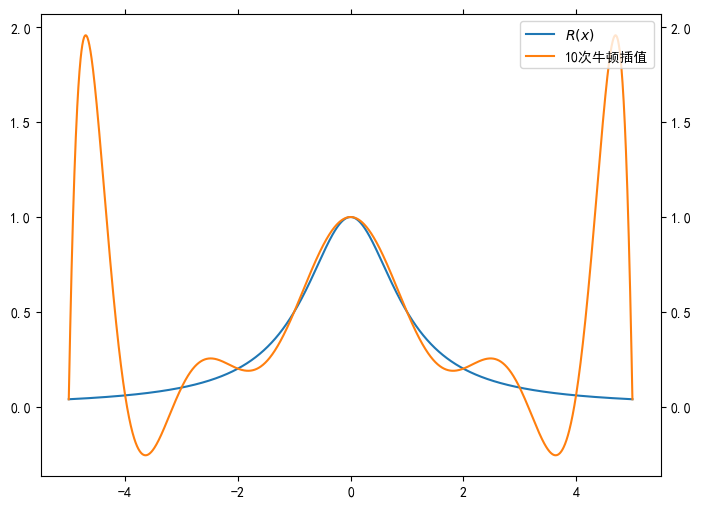
\includegraphics{pics/P3.2.png}
        \caption{问题二图像对比}
        \label{graph:1}
        \end{figure}
    可以看出,在中间部分Newton插值多项式的逼近效果较好,但在两端出现了很大的震荡,原因在于插值点的选取是等距的,而多项式的次数较高(10次),所以会出现Runge现象,即在两端有较大的误差. 与图一20次Lagrange插值多项式(不等距基点)的图像形成了对比.
\section{问题三}
    \subsection[short]{问题}
    用等距节点$x_i=-5+i, i=0,1,...,10.$画出分段线性插值函数的图像;
    \subsection{算法思路}
    对于分段线性插值,只需记录插值点的横坐标与纵坐标,再逐点用直线段连接即可.\\ \indent
    可以通过Python的Scipy库中的\texttt{interpolate.interp1d}函数构造出分段线性插值多项式.
    \subsection{结果分析}%重点(误差图、结果图、分析算法的收敛性(速度)、内存使用(时间、空间)、计算量、稳定性
    \begin{figure}[H]
        \centering
        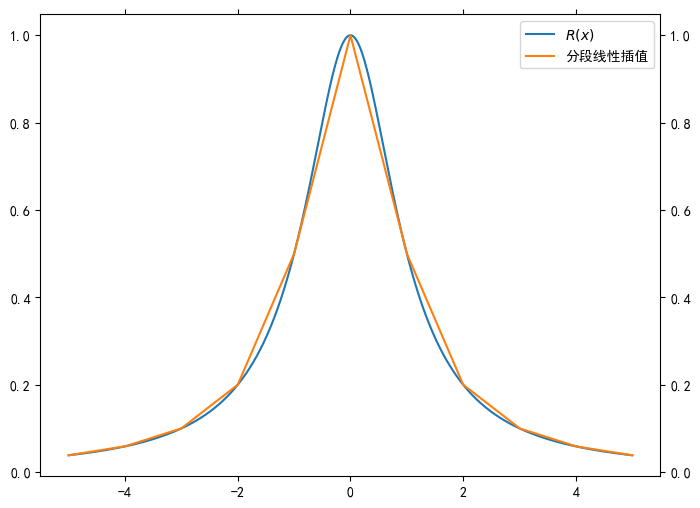
\includegraphics{pics/P3.3.png}
        \caption{问题三图像对比}
        \label{graph:1}
        \end{figure}
    可以看出,在原函数导数的绝对值较小的部分,线性插值的效果较好,而在原函数导数绝对值较大的部分,线性插值的误差较大.
\section{问题四}
    \subsection{问题}
    用等距节点$x_i=-5+i, i=0,1,...,10.$画出三次自然样条插值函数的图像;
    \subsection{算法思路}
    记$m_i=S^{''}(x_i),\;h_i=x_{i+1}-x_i$,则每一个小区间上的函数$S_i(x)$由以下公式给出:
    \begin{align}
        S_i(x)=\dfrac{1}{h_i}[\dfrac{m_i}{6}(x_{i+1}-x)^3+\dfrac{m_{i+1}}{6}(x-x_i)^3]+f(x_i)+f[x_i,x_{i+1}](x-x_i)-\dfrac{{h_i}^2}{6}[(m_{i+1}-m_i)\dfrac{x-x_i}{h_i}+m_i]
    \end{align}
    于是可先计算出二阶均差表,再计算$m_i$,只需解下述线性方程组:
    \begin{equation*}
        \left(
        \begin{matrix}
        2h_1 & h_1       &  & &\\
        h_1  & 2(h_1+h_2)& h_2\\
             & h_2       & 2(h_2+h_3) &h_3     &  &\\
             &           & \ddots     &\ddots  & \ddots &\\
             &           &            & h_{n-1}& 2(h_{n-1}+h_n) & h_n\\
             &           &            &        & h_n            &2h_n\\
        \end{matrix}
        \right)
        \left(
        \begin{matrix}
        m_1\\
        m_2\\
        \vdots \\
        \vdots \\
        m_n\\
        m_{n+1}
        \end{matrix}
        \right)=6
        \left(
        \begin{matrix}
        d_1\\
        d_2\\
        \vdots \\
        \vdots \\
        d_n\\
        d_{n+1}
        \end{matrix}
        \right)
    \end{equation*}
    其中
    \begin{align*}
         &d_1=f[x_1,x_2] \\
         &d_i=f[x_i,x_{i+1}]-f[x_{i-1},x_i],\quad i=2,\cdots,n\\
         &d_{n+1}=-f[x_n,x_{n+1}]
    \end{align*}
    (1)式可改写为
    \begin{align}
        S_i(x)=\sum_{k=1}^4 A_{k,i}(x-x_i)^{k-1},\;x\in [x_i,x_{i+1}]
    \end{align}
    其中
    \begin{align*}
        A_{1,i}&=f(x_i),\\
        A_{2,i}&=f[x_i,x_{i+1}]-\dfrac{h_i}{6}(m_{i+1}+2m_2),\\
        A_{3,i}&=\dfrac{m_i}{2},\\
        A_{4,i}&=\dfrac{m_{i+1}-m_i}{6h_i}
    \end{align*}
    已知$f[x_i,x_{i+1}],m_i,d_i,h_i$,即可按照(2)式用三重循环计算出$S_i(x)$在若干所需作图点的值.\\ \indent
    可以通过Python的Scipy库中的\texttt{interpolate.CubicSpline}函数构造出自然三次样条插值多项式.
    \subsection{结果分析}%重点(误差图、结果图、分析算法的收敛性(速度)、内存使用(时间、空间)、计算量、稳定性
    \begin{figure}[H]
        \centering
        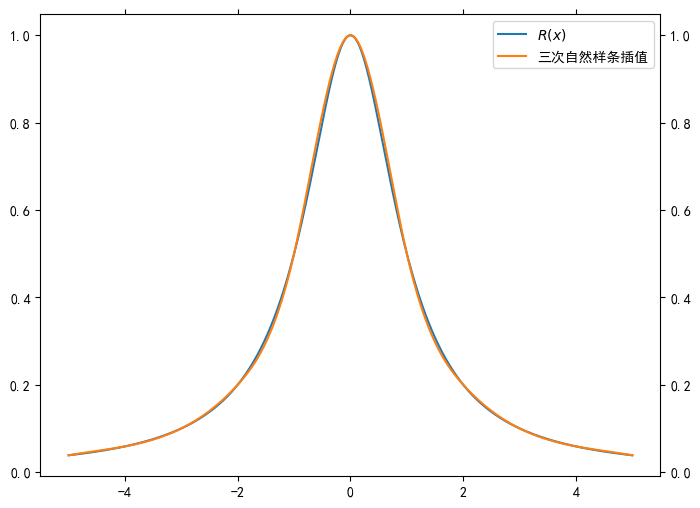
\includegraphics{pics/P3.4.png}
        \caption{问题四图像对比}
        \label{graph:1}
        \end{figure}
    可以看出,自然三次样条插值的逼近效果在整个区间上都很好.
\section{问题五}
    \subsection{问题}
    用等距节点$x_i=-5+i, i=0,1,...,10.$画出分段三次Hemite插值(相邻两点的函数值和一阶导数值)函数的图像.
    \subsection{算法思路}
    根据相邻两点的函数值和一阶导数值,可以在每个区间上得到三阶Hermite插值多项式$H_3(x)$:
    \[
        H_3(x)=\sum_{i=0}^1[1-2(x-x_i){l_i}^{'}(x_i)]{l_i}^2(x)+\sum_{i=0}^1 f^{'}(x_i)(x-x_i){l_i}^2(x)
    \]
    其中
    \begin{align*}
        l_i(x)&=\prod_{\substack{j=0\\j\neq i}}^n \dfrac{x-x_i}{x_i-x_j},\quad i=0,1\\
        l_i^{'}(x)&=\dfrac{1}{x_i-x_j},\quad i=0,1,\;j\neq i 
    \end{align*}
    利用上述公式,可以类似地用两重循环求得Hermite多项式在若干所需作图点的值.\\ \indent
    可以通过Python的Scipy库中的\texttt{interpolate.PchipInterpolator}函数构造出分段三次Hermite插值多项式.
    \subsection{结果分析}%重点(误差图、结果图、分析算法的收敛性(速度)、内存使用(时间、空间)、计算量、稳定性
    \begin{figure}[H]
        \centering
        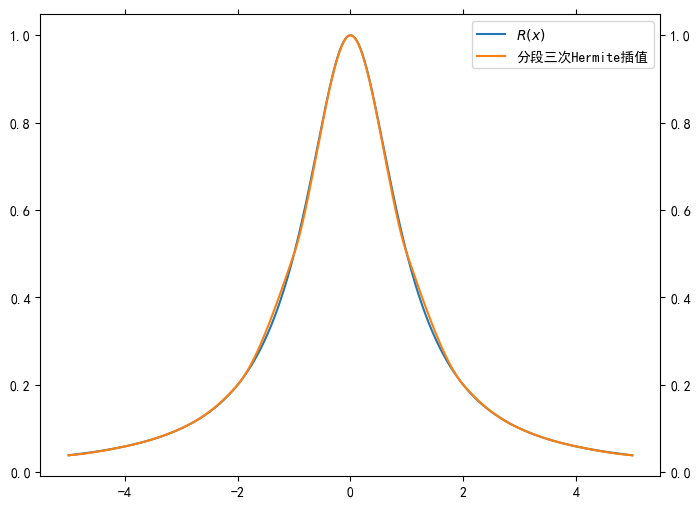
\includegraphics{pics/P3.5.png}
        \caption{问题五图像对比}
        \label{graph:1}
        \end{figure}
    可以看出,Hermite插值的逼近效果在整个区间上都很好,几乎和原函数重合.
\section{结论}
    \begin{figure}[H]
        \centering
        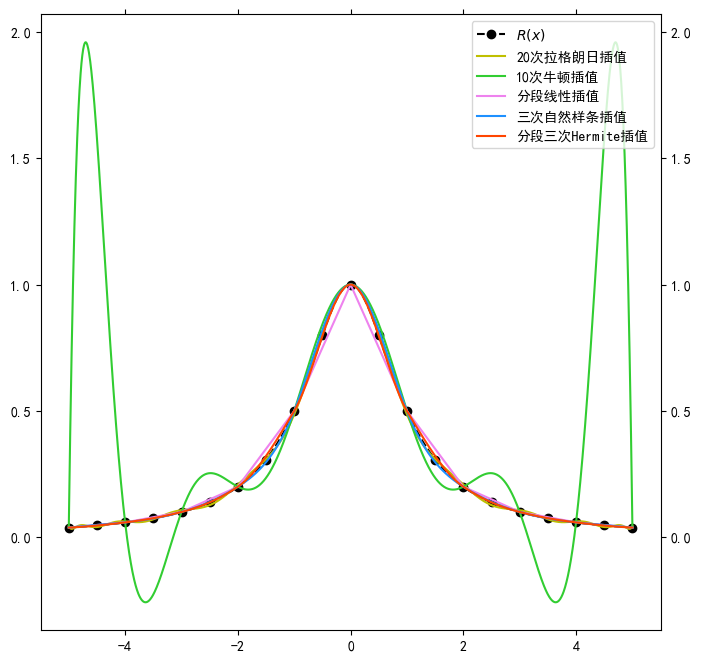
\includegraphics{pics/P3.6.png}
        \caption{全部插值函数图像对比}
        \label{graph:1}
        \end{figure}
\;对比上述五种插值方法的效果,可以得出以下结论:
\begin{enumerate}
    \item 在进行Lagrange插值和Newton插值时,对于次数较高的情形要避免等距基点的情况,否则在端点附近会出现Runge现象,误差较大.
    \item 分段线性插值在计算时很方便,但若得到更好的逼近效果,则需要增加插值点的个数.
    \item  三次样条插值和分段Hermite插值的效果要明显优于Newton插值和Lagrange插值.
    \begin{figure}[H]
        \centering
        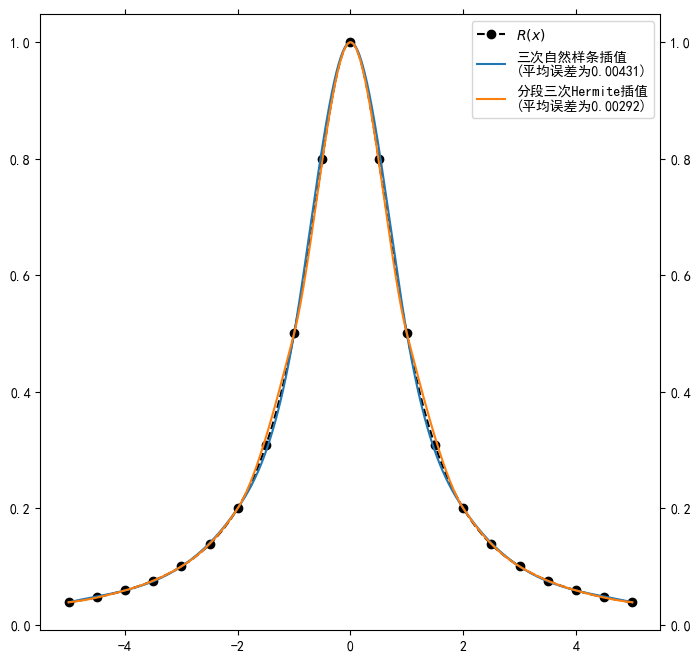
\includegraphics{pics/P3.7.png}
        \caption{三次样条插值与分段Hermite插值图像对比}
        \label{graph:1}
        \end{figure}
    \item 三次样条插值和分段Hermite插值各有优劣:一方面,三次样条插值保证了插值函数在这个区间上是二阶连续可微的,而分段Hermite插值不能保证在相邻小区间公共点处二阶可导;另一方面,在本例中,分段Hermite插值的逼近效果要略优于三次样条插值.
\end{enumerate}
\clearpage

\section{附录: 程序代码}
\rmk 所有题目共用一个.ipynb源文件.
\lstset{
    numbers=left,
    language=Python,
    keywordstyle=\color{blue!100},
    commentstyle=\color{green!50!blue!50!},
    frame=shadowbox,%阴影
    escapeinside='',%英文分号输入中文
    xleftmargin=2em,xrightmargin=2em,aboveskip=1em,
    framexleftmargin=2em,
    extendedchars=false}

\begin{lstlisting}[aboveskip=0pt]
import numpy as np
import matplotlib.pyplot as plt
from scipy.interpolate import lagrange, interp1d, 
CubicSpline, PchipInterpolator
#display Chinese in figures
plt.rcParams['font.sans-serif'] = ['SimHei']
plt.rcParams['axes.unicode_minus'] = False
%matplotlib inline
\end{lstlisting}
\begin{lstlisting}[aboveskip=0pt]
# 定义 R(x) 函数
def R(x):
    return 1 / (1 + x**2)

# 定义节点
n_lagrange = 21
n_newton = 11
x_lagrange = [5 * np.cos((2 * i + 1) / (42) * np.pi) for i in range(n_lagrange)]
x_newton = [-5 + i for i in range(n_newton)]
\end{lstlisting}
\begin{lstlisting}[aboveskip=0pt]
# 定义 Lagrange 插值多项式
def lagrange_interpolation(x, x_nodes, y_nodes):
    poly = lagrange(x_nodes, y_nodes)
    return poly(x)
# 定义 Newton 插值多项式
def newton_interpolation(x, x_nodes, y_nodes):
    poly = lagrange(x_nodes, y_nodes)
    return poly(x)
\end{lstlisting}
\begin{lstlisting}[aboveskip=0pt]
# 计算插值多项式的值
x_values = np.linspace(-5, 5, 2001)
lagrange_values = lagrange_interpolation(x_values, x_lagrange, 
R(np.array(x_lagrange)))
newton_values = newton_interpolation(x_values, x_newton, R(np.array(x_newton)))
\end{lstlisting}
\begin{lstlisting}[aboveskip=0pt]
# 20次Lagrange插值多项式的图像
plt.figure(figsize=(10,6))
plt.tick_params(axis='both', which='both', bottom=True, top=True, left=True, 
right=True,labelright=True)
plt.plot(x_values, R(x_values), label='$R(x)$', color='blue')
plt.plot(x_values, lagrange_values, label='20次拉格朗日插值', color='red')
plt.legend(loc='upper right')
\end{lstlisting}
\begin{lstlisting}[aboveskip=0pt]
# 10次Newton插值多项式的图像
plt.figure(figsize=(10,6))
plt.tick_params(axis='both', which='both', bottom=True, top=True, left=True, 
right=True,labelright=True)
plt.plot(x_values, R(x_values), label='$R(x)$', color='blue')
plt.plot(x_values, newton_values, label='10次牛顿插值', color='red')
plt.legend(loc='upper right')
\end{lstlisting}
\begin{lstlisting}[aboveskip=0pt]
# 分段线性插值函数的图像
plt.figure(figsize=(10,6))
plt.tick_params(axis='both', which='both', bottom=True, top=True, left=True, 
right=True,labelright=True)
linear_interp = interp1d(x_newton, R(np.array(x_newton)), kind='linear', 
fill_value="extrapolate")
plt.plot(x_values, R(x_values), label='$R(x)$', color='blue')
plt.plot(x_values, linear_interp(x_values), label='分段线性插值', color='red')
plt.legend(loc='upper right')
\end{lstlisting}
\begin{lstlisting}[aboveskip=0pt]
# 三次自然样条插值函数的图像
plt.figure(figsize=(10,6))
plt.tick_params(axis='both', which='both', bottom=True, top=True, left=True, 
right=True,labelright=True)
cubic_spline = CubicSpline(x_newton, R(np.array(x_newton)))
plt.plot(x_values, R(x_values), label='$R(x)$', color='blue')
plt.plot(x_values, cubic_spline(x_values), label='三次自然样条插值', color='red')
plt.legend(loc='upper right')
\end{lstlisting}
\begin{lstlisting}[aboveskip=0pt]
# 分段三次Hermite插值函数的图像
plt.figure(figsize=(10,6))
plt.tick_params(axis='both', which='both', bottom=True, top=True, left=True, 
right=True,labelright=True)
pchip_interp = PchipInterpolator(x_newton, R(np.array(x_newton)))
plt.plot(x_values, R(x_values), label='$R(x)$', color='blue')
plt.plot(x_values, pchip_interp(x_values), label='分段三次Hermite插值', color='red')
plt.legend(loc='upper right')
\end{lstlisting}
\begin{lstlisting}[aboveskip=0pt]
import seaborn as sns
sns.set_theme(style="darkgrid")
# display Chinese in sns plot
plt.rcParams['font.sans-serif'] = ['SimHei']
# plot all curves in one gragh
plt.figure(figsize=(20,12))
plt.tick_params(axis='both', which='both', bottom=True, top=True, left=True, 
right=True,labelright=True)
plt.plot(x_values, R(x_values), label='$R(x)$', linestyle='--',color='black',
marker="o", markeredgecolor='black', markerfacecolor='black', markevery=100)
plt.plot(x_values, lagrange_values, label='20次拉格朗日插值', color='y')
plt.plot(x_values, newton_values, label='10次牛顿插值', color='limegreen')
plt.plot(x_values, linear_interp(x_values), label='分段线性插值', 
color='violet')
plt.plot(x_values, cubic_spline(x_values), label='三次自然样条插值', 
color='dodgerblue')
plt.plot(x_values, pchip_interp(x_values), label='分段三次Hermite插值', 
color='orangered')
plt.legend(loc='upper right')
\end{lstlisting}
\begin{lstlisting}[aboveskip=0pt]
plt.figure(figsize=(8,8))
plt.tick_params(axis='both', which='both', bottom=True, top=True, left=True, 
right=True,labelright=True)
plt.plot(x_values, R(x_values), label='$R(x)$', linestyle='--',color='black',
marker="o", markeredgecolor='black', markerfacecolor='black', markevery=100)
plt.plot(x_values, cubic_spline(x_values), label='三次自然样条插值\n
(平均误差为0.00431)')
plt.plot(x_values, pchip_interp(x_values), label='分段三次Hermite插值\n
(平均误差为0.00292)')
plt.legend(loc='upper right')
r1=(np.sum((np.abs(R(x_values)-cubic_spline(x_values)))))/2000
r2=(np.sum((np.abs(R(x_values)-pchip_interp(x_values)))))/2000
print(f'三次样条插值的平均误差为{r1}')
print(f'分段Hermite插值的平均误差为{r2}')
\end{lstlisting}
\clearpage


\clearpage

\bibliographystyle{unsrt}
\bibliography{Reference}
\end{document}